\section{Parallel I/O}

Input-output could be a serious bottleneck if we do not pay the right attention.
In particular, when dealing with supercomputers, two major problems arise:
\begin{itemize}
\item needing of parallel I/O,
\item avoid endianness problem related.
\end{itemize}
As first thing let us introduce I/O.\par
In computer architecture, the combination of the CPU and main memory, to which the CPU can read or write directly using individual instructions, is considered the brain of a computer. Any transfer of information to or from the CPU/memory combo, for example by reading data from a disk drive, is considered I/O~\cite{io}.
When dealing with cluster the transit of data from disk to CPU is not so straightforward. The presence of multiple CPU require the adoption of one of the following strategies.\par
\begin{wrapfloat}{figure}{l}{0pt}
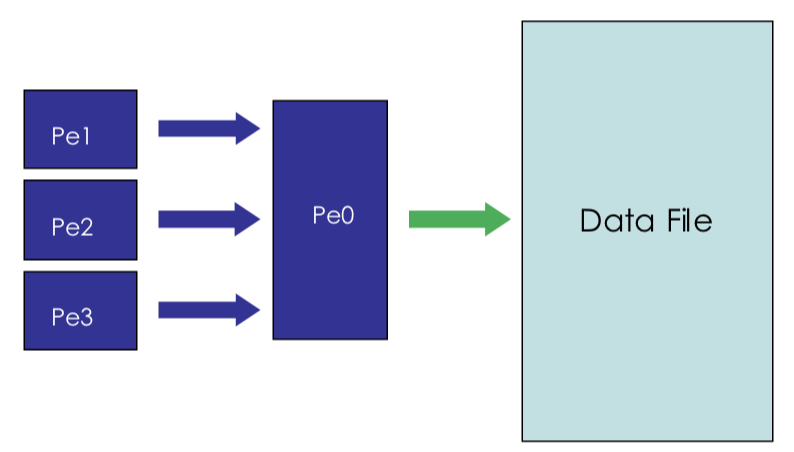
\includegraphics[width=0.5\textwidth]{grafici/masterslave}
\caption{Master-Slaves I/O setup}
\end{wrapfloat}
The most basic strategy is called ``Master-Slave''. In this kind of strategy a single node of the grid have access to the storage, therefore no scalability is provided. The slave nodes must send/receive data from the master, therefore we face strong slowdown related to the huge workload required to perform I/O by the single node and the following communications among nodes.\\

\begin{wrapfloat}{figure}{r}{0pt}
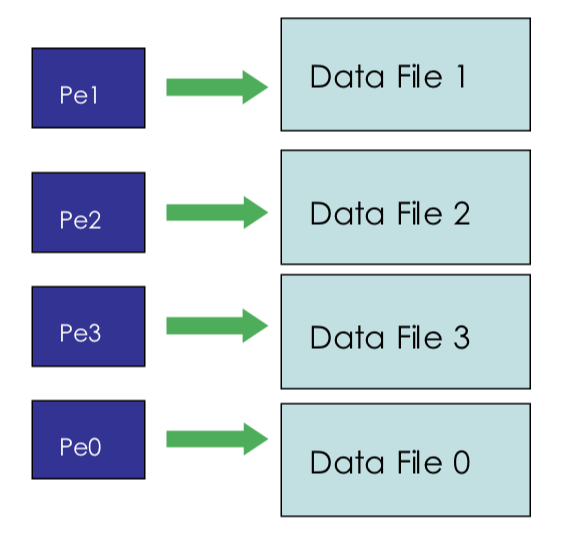
\includegraphics[width=0.5\textwidth]{grafici/localio}
\caption{Distributed I/O on local files}
\end{wrapfloat}
\par
The setup shown here beside perform distributed I/O on local files. Such kind of implementation is scalable, ensure data consistency and avoid communication during I/O phase. However, since every processor writes data on its own hard storage, it require a great deal of post processing work to glue data among each others, which increase linearly with the number of nodes. For this reason we can not consider it affordable. \\

\begin{wrapfloat}{figure}{r}{0pt}
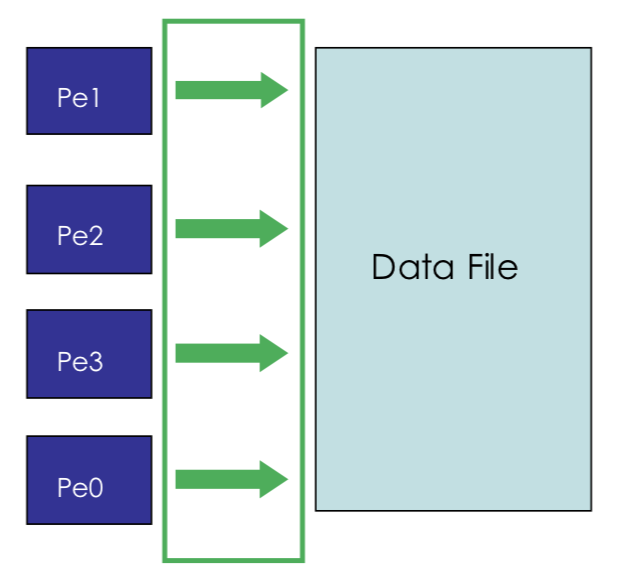
\includegraphics[width=0.5\textwidth]{grafici/mpiio}
\caption{Coordinated controlled accesses}
\end{wrapfloat}
\par
The last kind of I/O setup, which is the most updated and optimized, is the so called coordinated controlled accesses.
Scalability reaches its peak with this kind of implementation, which takes care of possible communications needing by its own.
In this approach every CPU can access to the single storage memory in which the dataset is hosted, and in concomitancy with the other processes, writes the data. As can be understood, the reading/writing operation is intrinsically fragile, since guarantee data consistency can be hard. To avoid consistency lacks, the MPI-IO has been introduced with the deployment of MPI-2 standard~\cite{MPI:standard2}.

On top of MPI-IO several high level I/O libraries arose, two well established examples are parallel netCDF and parallel HDF5. 

At exception of the Master-Slave approach, every presented strategy require the adoption of a parallel file system.
In computing, a file system or filesystem controls how data is stored and retrieved. Without a file system, information placed in a storage medium would be one large body of data with no way to tell where one piece of information stops and the next begins. By separating the data into pieces and giving each piece a name, the information is easily isolated and identified. We can briefly define the file system as the structure and logic rules used to manage the groups of information and their names.
In the same fashion a parallel file system maintains logical space and provides efficient access to data for distributed memory configurations.\\
\par
Let us establish the concept of endianness.
Intel introduces their white paper with the following sentence:\par
``Endianness describes how multi-byte data is represented by a computer system and is dictated by the CPU architecture of the system. Unfortunately not all computer systems are designed with the same Endian-architecture. The difference in Endian-architecture is an issue when software or data is shared between computer systems''\cite{endianness}.\par
Since our binary database has been built on Marconi, at Cineca, but the post-processing analysis take place on our personal computers, we need to guarantee results portability with a reliable method to store the data. \\
\par
Unfortunately MPI-IO can not set a bit ordering different from the machine's natives ones, and we can not assure portability in this way. To do so we have to move from MPI-IO to a library capable to satisfy our requirements.\par
Employ the well established parallel HDF5 library is the natural choice.



\subsection{Parallel HDF5 Library}
Hierarchical Data Format 5, or HDF5~\cite{hdf5}, is widespread scientific data format used by many application to deal with large sets of data. Parallel Hierarchical Data Format 5, or pHDF5, is the parallelized version for clusters.\par
Designed to store and organize large amounts of data, HDF5 has been originally developed at the National Center for Supercomputing Applications. 
The crucial feature is its ability to store binary dataset in a processor independent fashion, guaranteeing the portability of the data. This allows extremely compact file dimensions, since we are dealing with binary data, and in the same time we can exploit the advantages of ASCII encoding.
The hierarchical file ordering allows to define a Linux like environment made up of root folder, subfolders, tables, figure, attributes, links and others useful things to maintain the database as readable as possible.\par
The price for the high flexibility of such data format is the impossibility to have a plug and play VTK reader. In fact we have to rely on third party software to instruct the VTK tool, in our case Paraview, to inspect the database. \par
We decide to use XDMF3~\cite{xdmf3}, acronym of eXtensible Data Model and Format 3, to generate and XML file to put beside our HDF5 file, so that Paraview, or any other VTK software, use to read the database.

